\section{Thrust 3. Predictive Execution}
\label{sec:thrust3}

\subsection{Key Ideas}

In this work, we advocate for an emerging execution paradigm that we
call {\bf predictive execution}, PredEx. In predictive execution,
similar to the traditional execution, a program is provided with
specific input value. However, the execution is not carried out with
the computer performing the instructions in the program. Instead, a
trained machine learning (ML) model predicts the execution step based
on the specific input value. As a result, the execution path
corresponding to the input is derived. Predictive execution offers
several benefits in different usage scenarios in software development.

First, predictive execution is particularly useful in the scenarios
that the actual execution requires a dedicated environment or
hardware, thus, becomes prohibitively challenging. 

Second, predictive execution can serve as a building block for the
execution of incomplete code snippets, which are rendered as
inexecutable. By predicting the execution steps of inexecutable code,
it becomes possible to detect potential bugs early on. This
application could be particularly useful for identifying problematic
code snippets in online forums like StackOverflow, where there may be
instances of vulnerable code that can be migrated to a
codebase~\cite{verdi-tse22}. Such early detection avoids wasting
effort from developers to integrate the inexecutable code snippets
from online forums into a project.

Third, in software testing, by predicting the execution path
corresponding to an input, we can estimate code coverage without
executing every test case in the test
suite~\cite{ball-toplas94,elbaum-icsm01}. This is crucial for
debugging in security contexts, where executing untrusted code could
lead to vulnerabilities or system compromises. Predictive execution
allows for the analysis of potentially harmful or untrusted
code. Thus, the potential risks associated with running unverified or
potentially malicious code are mitigated.

%In the context of fuzz testing~\cite{fuzzing-testing-survey-2020},
%where test cases are generated automatically to explore program
%faults, predictive execution can help determine if a newly generated
%test satisfies the conditions required by a fuzzing engine to exercise
%a particular path. This capability allows for a more targeted and
%efficient model to fuzzing, potentially leading better bug
%detection. Moreover, with the predicted code coverage, fault
%localization can be enabled for those cases.

%In pursuit of predictive execution, the state-of-the-art
%approaches~\cite{liu2023code,ding2023traced} aim to predict execution
%traces and associated variable values along the way. However, they
%exhibit certain key limitations. TRACED~\cite{ding2023traced} does not
%handle well the code featuring iterative structures, while
%CodeExecutor~\cite{liu2023code} does not perform well for the
%execution with runtime errors and control flow statements (such as
%\code{return}, \code{break}, \code{continue}). The precision in
%predicting execution traces remains modest. We observed that these
%approaches place a substantial burden on models to grasp the
%transformation patterns from the entire program and input values to
%the full execution traces.

We propose a novel approach called {\bf PredEx} for predictive execution, which predicts the execution trace of a Python program based on its input. We design a new technique called {\bf blended analysis}, combining the strengths of both {\em Static Program Analysis} (PA) and {\em Large Language Models} (LLMs) to predict the next executed statement and execution trace given a Python program and its input. While LLMs like GPT-3.5~\cite{GPT3.5}, CodeT5~\cite{wang2023codet5}, Code Llama~\cite{code_llama}, 
%RoBERTa{liu2019roberta},
and others have demonstrated proficiency in comprehending source code,
their direct application in predicting execution traces for an entire
program with its input is constrained by various dynamic intricacies
of code execution. Conversely, while static PA can have a
correct~solution in some task, it tends to overestimate the actual
paths taken during execution.

\subsection{Predictive Execution Algorithm via Blended Analysis between PA and ML}

\begin{wrapfigure}{r}{0.6\textwidth}
%\begin{figure*}[t]
\begin{center}
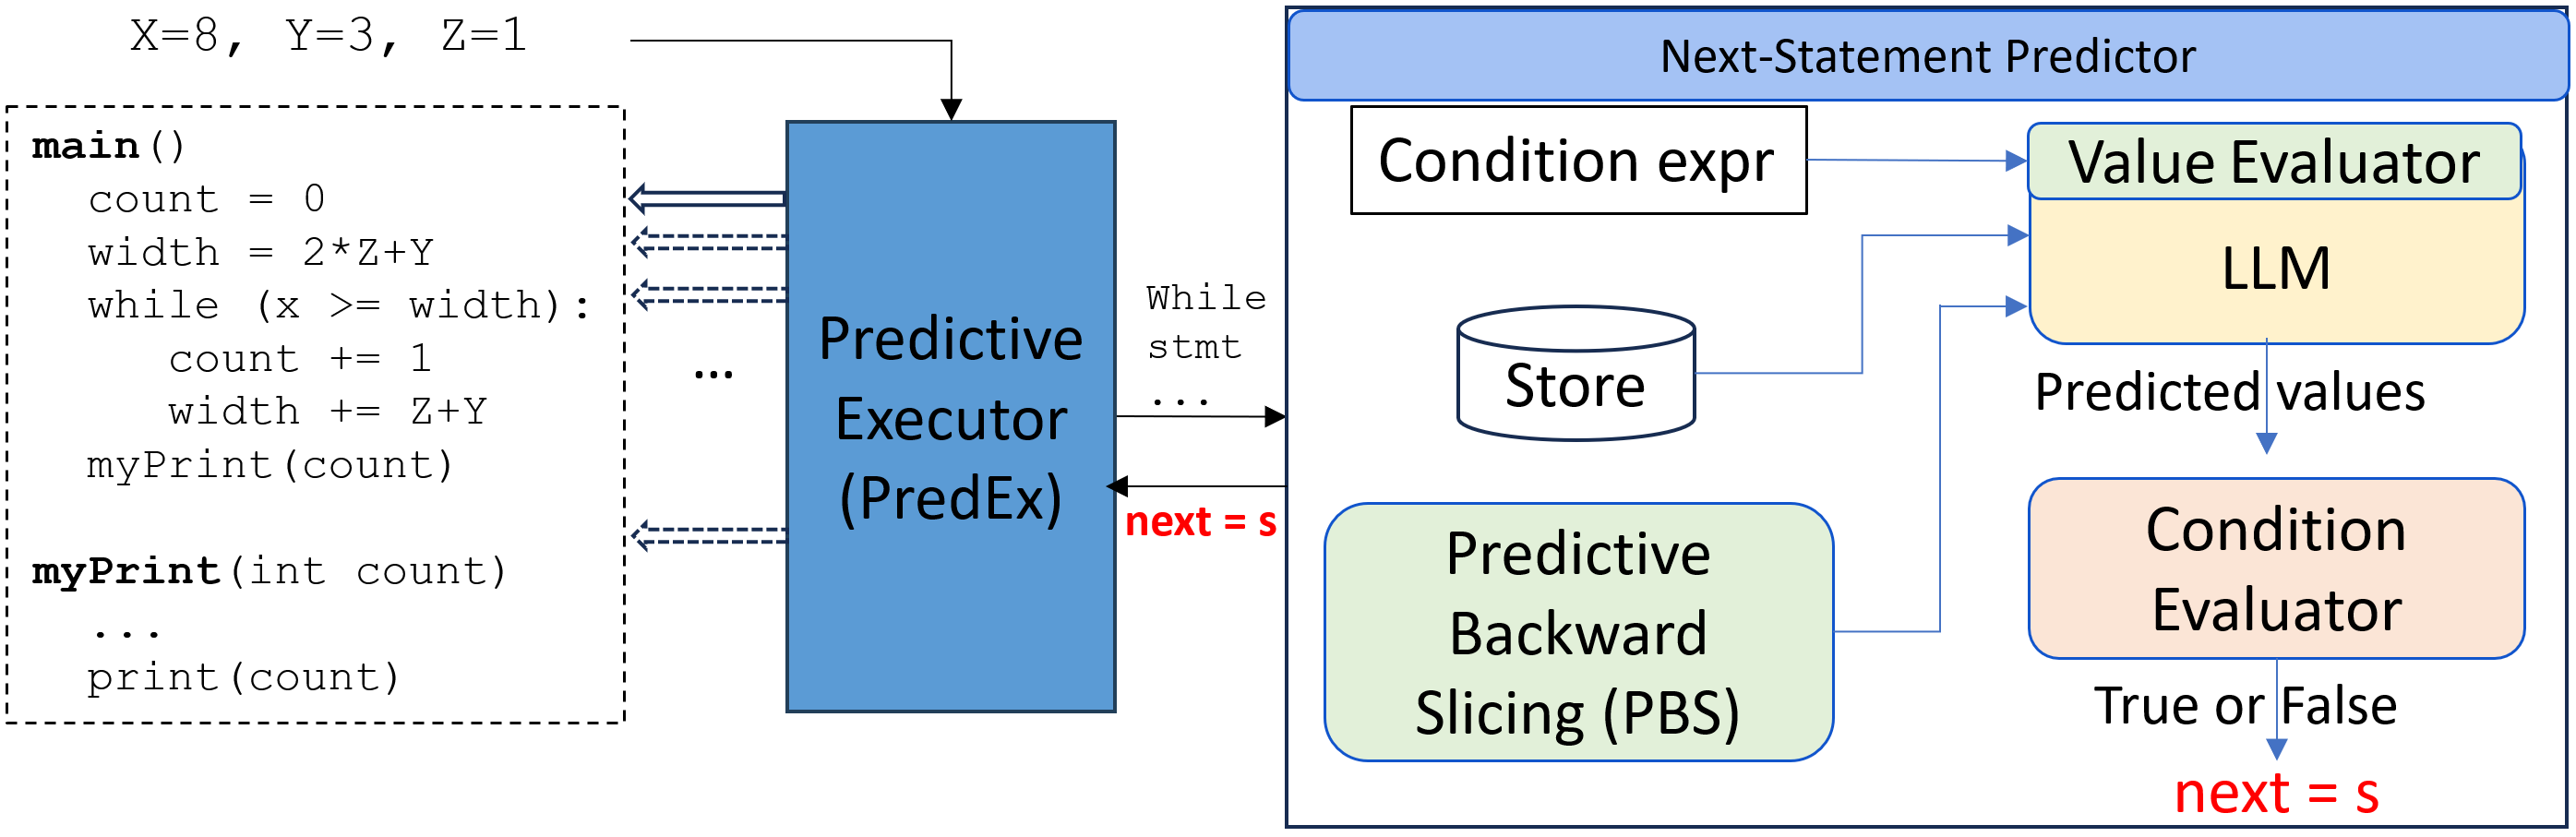
\includegraphics[width=4in]{overview-4.png}
\vspace{-22pt}
\caption{PredEx: Blended Analysis Framework for Predictive Execution}
\label{fig:overview}
\end{center}
%\end{figure*}
\end{wrapfigure}

In blended analysis, we decompose the original problem into smaller sub-tasks and allocate~each task to either PA or LLM based on their respective strengths. At the coarse-grained level, we divide the predictive execution problem into predicting the next executed statement at each step. When PA can make deterministic decisions, such as determining the next executed statement within a block, we leverage PA for that to alleviate the potential inaccuracy of the LLM. However, when PA is unable to ascertain the execution flow, particularly at branching points (e.g., \code{if}, \code{while}, \code{for}, etc.), we enlist the LLM to handle tasks critical for the decisions at those branching points. At the fine-grained level of the task of LLM-based branching decisions, we also harness PA to assist the LLM in focusing on the pertinent statements when making decisions about the branching direction. That is, we posit that by providing the LLM with support from PA and feeding it relevant statements, we can guide it in reasoning about the execution of a smaller subset of statements without executing them. Via pre-training, LLMs have learned patterns, logic, and reasoning capabilities that enable them to predict program execution for a smaller set of statements relevant to branching decisions.

%=====================================================
Specifically, the two sub-tasks at a branching point for the LLM
include {\em value evaluator} and {\em condition evaluator}. First, the value
evaluator focuses on determining the values of variables involved in
decision-making at a branching point. By using backward slicing
starting from those variables, we can help the LLM focus only on the
relevant, important statements that influence the values of the
variables. We build the backward slices and use the current predicted
statements and paths in the trace to approximate the dynamic backward
slice. Let us call it {\em predictive backward slice}. By such slices
and predicted values, we enable the LLM to recognize patterns and
dependencies in the code that affect the values of the current
variables. By training the LLM via few-shot learning on the external
API calls, we enable it to derive the output values of such calls.
Second, the condition evaluator, builds on the values obtained from
the value evaluator. Given the values of the variables at a branching
point, the condition evaluator can predict the outcome of the
condition expression. For this evaluation, one can have different
strategies. First, one can leverage the LLM as in the value
evaluator. Second, one can leverage the expression evaluator. Third,
one could build his/her own probabilistic condition evaluator to
estimate the probability of the condition being true.



%Fig.~\ref{fig:overview} shows an overview of PredEx. It accepts a
%Python program and input values. Its output is the predictive
%execution trace, i.e., the order of the statements that would be
%executed. The principle in PredEx is a {\bf blended analysis} between
%{\bf program analysis} and {\bf Large Language Model (LLM)}. The
%blended analysis is expressed in two folds. \underline{First}, when PredEx is
%certain on the execution order of the next statement $s$ based on the
%current statement, it will add $s$ into the resulting predictive
%execution trace. Only when it is not certain, e.g., at a branch of an
%\code{if} statement with an uncertain condition, PredEx requests its
%next-statement predictor (NSP) to provide the prediction of the
%potential next statement. \underline{Second}, even though we leverage LLM to
%predict the values of relevant variables and sub-expressions in the
%condition expression of a statement with a branching instruction, we use
%{\bf program analysis}, specifically the {\bf predictive backward slicing},
%to help the LLM pay attention only to the statements that might affect
%the evaluation of the condition. The backward slice for a variable
%might be long, thus, we design a strategy to optimize and shorten the
%slice by storing the predicted values of relevant variables at the
%latest prediction~point.

%With the blended analysis, we break down the task of predicting the
%execution into a smaller sub-tasks and leverage the deterministic
%nature of some sub-tasks (e.g., unconditional execution). We expect to
%help the LLM better decide the next executed statement.  In fact, in
%our empirical evaluation, PredEx improves over the state-of-the-art
%approaches, GPT-3.5~\cite{ChatGPT} and CodeExecutor~\cite{liu2023code},
%in which the source code and input are fed into the LLM to produce the
%entire execution trace.

\subsection{Predictive Execution: Illustrating Example}
\label{sec:example}

%\begin{figure}[htp]

\begin{wrapfigure}{r}{0.5\textwidth}
%\begin{figure}[t]  
\begin{center}
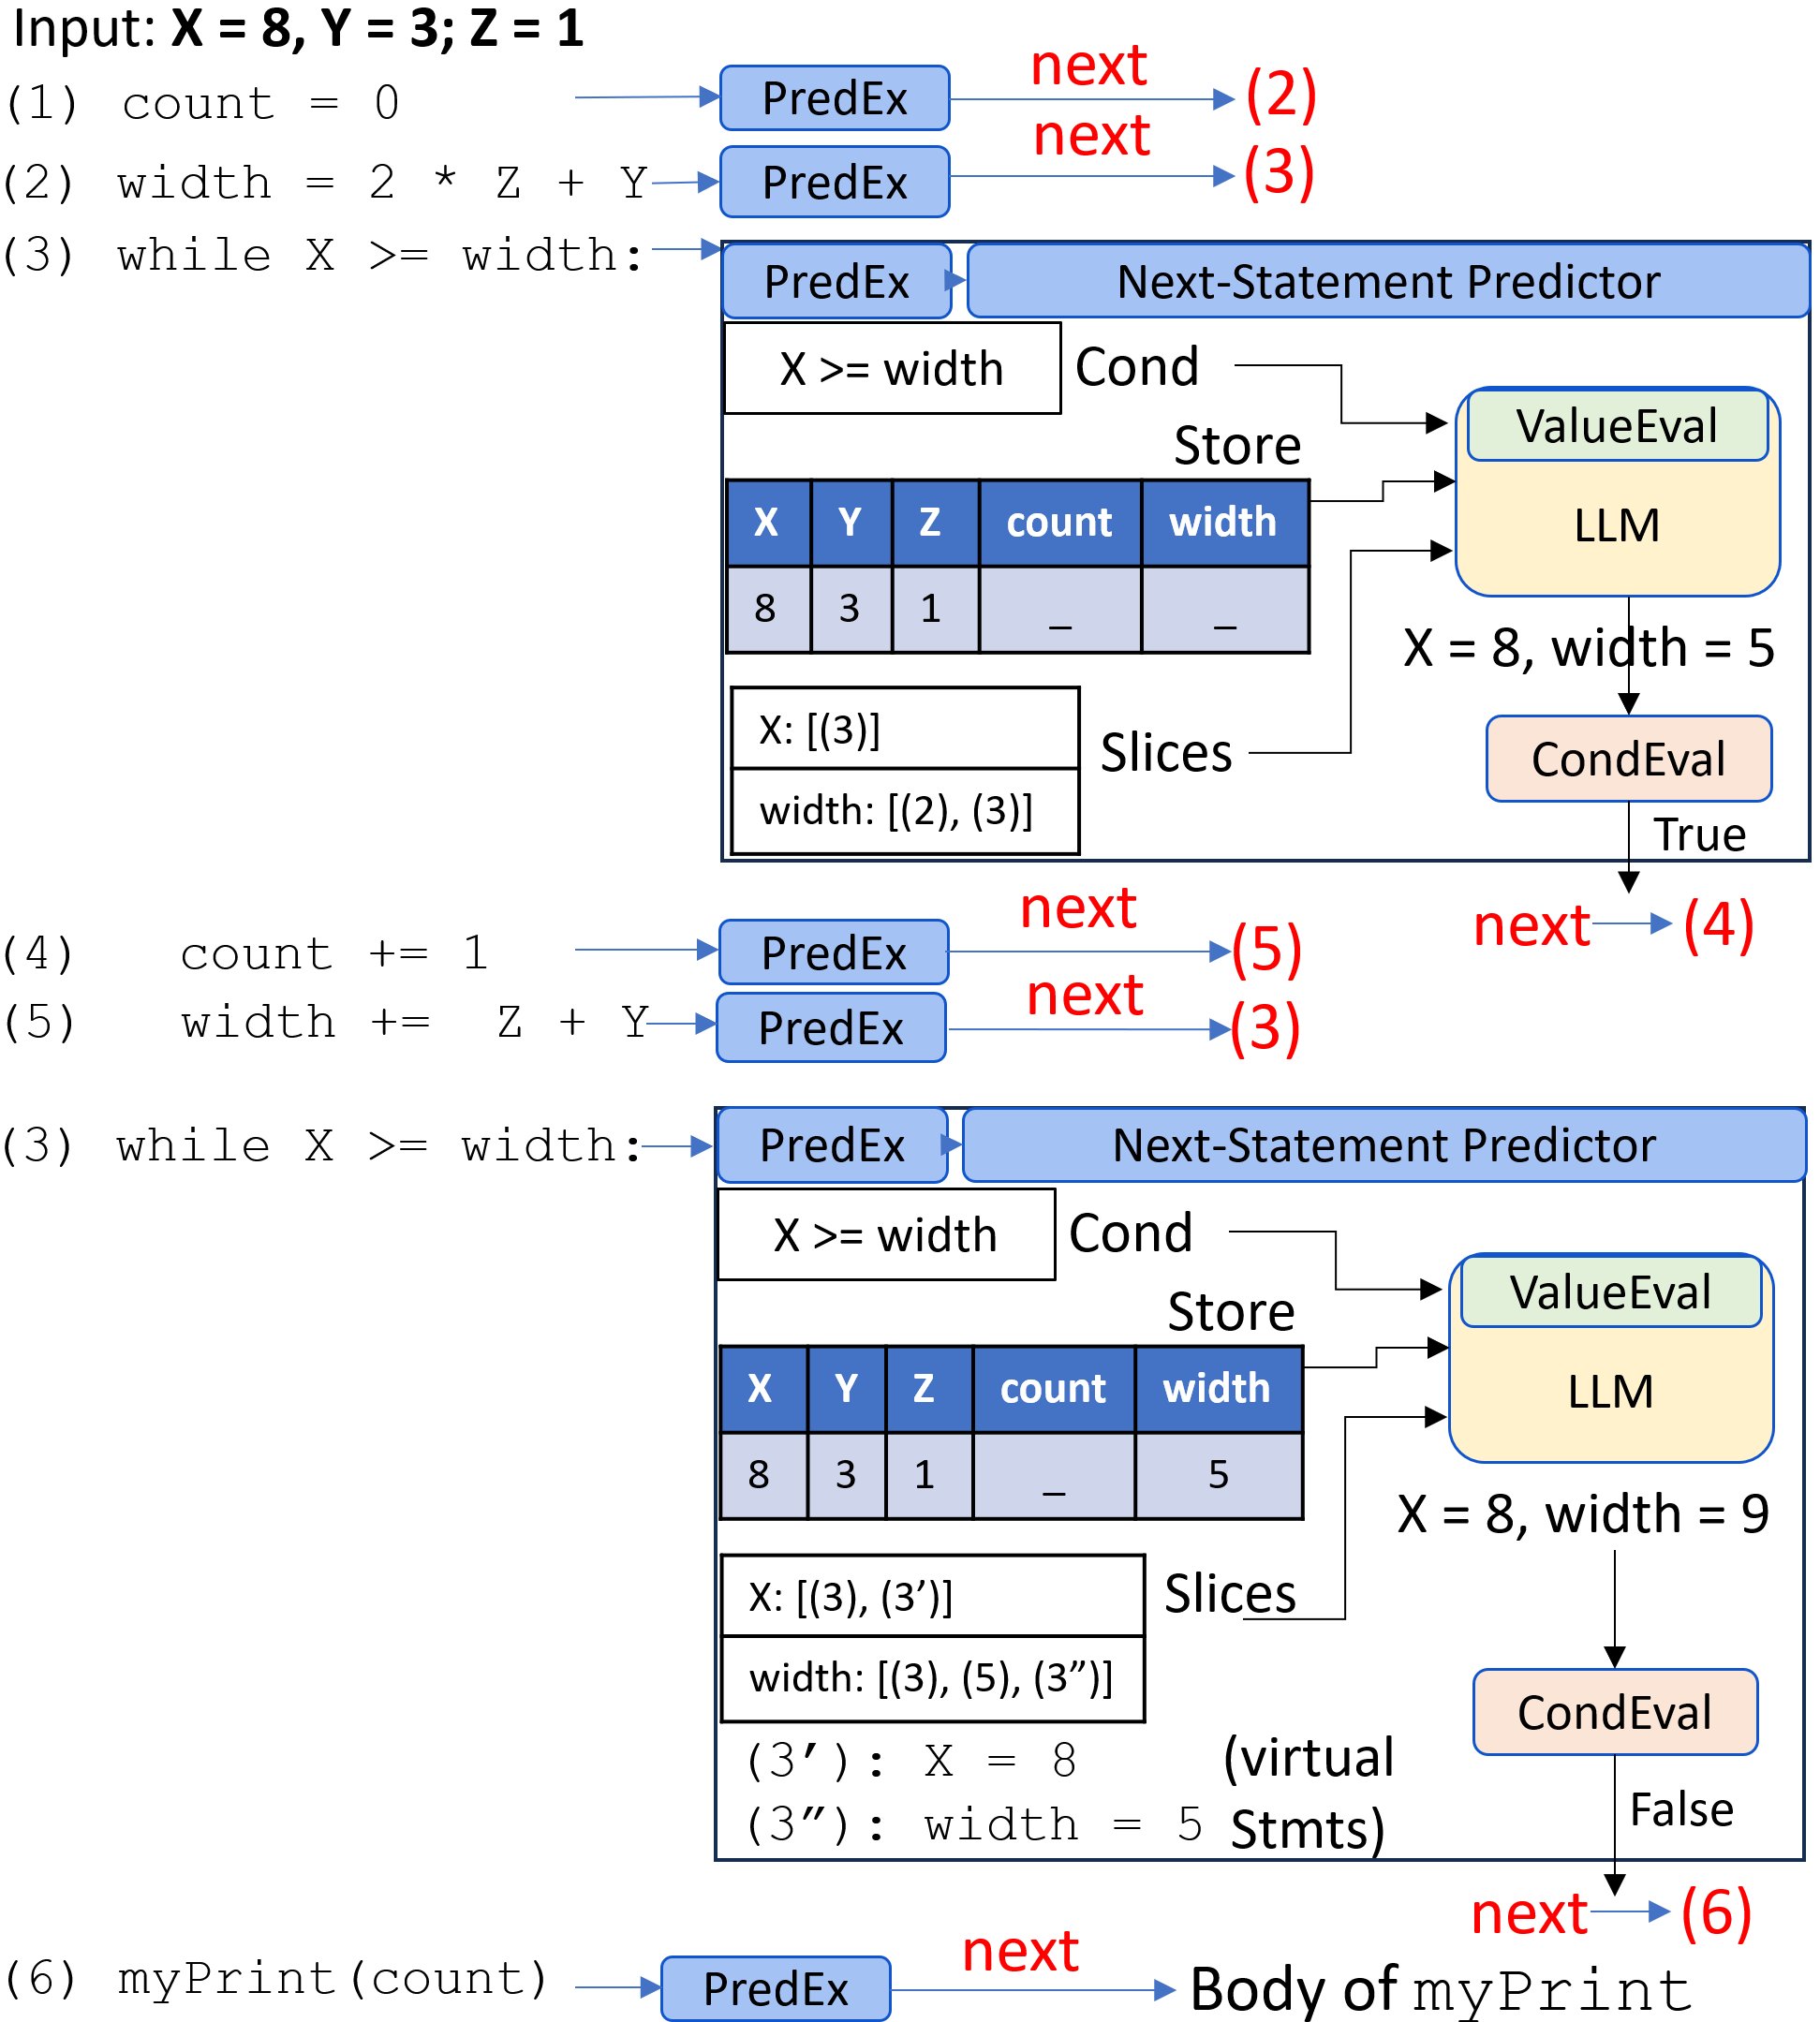
\includegraphics[width=3.2in]{example-4.png}
\vspace{-13pt}
\caption{Predictive Execution: An Illustrating Example}
\label{fig:illustration}
\end{center}
%\end{figure}
\end{wrapfigure}

Fig.~\ref{fig:illustration} illustrates how PredEx works on our
motivating example. For brevity in the figure, we use the new input
\code{X}=$8$, \code{Y}=$3$, and \code{Z}=$1$. Assume that, PredEx
starts with the assignment at line (1). Because line (1) is a simple
statement, PredEx decides the statement (2) to be the next
one. Similarly, PredEx decides the statement (3) as the one after
that.

At line 3, encountering a \code{while} statement, PredEx passes the
information on to the next-statement predictor. This LLM-based value
evaluator requires three pieces of information as
input. First, PredEx extracts the condition expression \code{X >=
  width}. Second, the current state of the value store $\theta$ includes the
initial values for the variables \code{X}=$8$, \code{Y}=$3$, and \code{Z}=$1$, and
the undefined values for \code{count} and \code{width} because those are the
values from the latest prediction point (also referred to as {\em
  check point}). If there is no prediction point yet, the latest check
point is at the very beginning. Third, PredEx computes two predictive
slices for the two variables involving in the condition
\code{X>=width}. The slice for \code{X} includes only the statement at line
(3), while the slice for \code{width} includes two statements at line (2)
and line (3).

From the three pieces of information, the LLM-based value evaluator
predicts the values of \code{X}=$8$ and \code{width}=$5$. After the store is
updated, the condition evaluator
will use it to evaluate \code{X>=width} and return $True$. To reduce
the number of requests to the LLM to update the values for all
variables, we only update the values of the variables involving in the
condition. For example, the value of the variable \code{count} is not
updated. The next prediction for the second iteration
will use the updated values in the store $\theta$. Because the
condition is predicted as $True$, the next-statement predictor will
return the statement (4) as the one.
%
Because the statement (4) is simple, PredEx decides the
statement (5) as the next one. Similarly, it moves on to
the statement (3) after that.



At the second iteration for the \code{while} statement at line 3,
PredEx also utilizes the next-statement evaluator. The condition is
the same: \code{X>=width}. However, the store $\theta$ is updated with
the latest predicted values: \code{X}=$8$, \code{Y}=$3$, \code{Z}=$1$,
\code{count}=$\_$, and \code{width}=$5$. To compute the backward
slices for \code{X} and \code{width}, PredEx performs differently
from the last time. Because in the previous prediction point, \code{X}
was evaluated to 8 and \code{width} was evaluated to 5, we create two
virtual statements: 1) statement (3'): \code{X}=$8$, and 2) statement
(3''): \code{width}=$5$ at the beginning of the loop (right after the
statement (3)). The predictive backward slice for \code{X} is computed
as containing the statement (3) and the new one (3'). Due to the new
virtual statement with the updated value of \code{width}, we only need
to include into the predictive backward slice for \code{width} the
statement (3), (5), and (3''). We do not need all the statements from
the beginning up to that point. That is, we do not include the
statement (2) into the PBS for \code{width} at this iteration.

With the condition \code{X>=width}, the store $\theta$, and the above
slices, the LLM-based value evaluator predicts the values \code{X}=$8$
and \code{width}=$9$. At this iteration, the condition evaluator
returns $False$, and the next statement is the statement (6), i.e.,
the loop ends.  For statement (6), PredEx will move on to
\code{myPrint()}.

%The statement (6) is an expression statement, which is an expression
%in the form of a function call to \code{myPrint(...)}. PredEx will
%move on to make prediction for the statements in the body of the
%\code{myPrint} function. The process continues until the end or
%\code{ERROR} occurs.
